\section{Introduction}

At some point in their academic journey, every student faces the challenge of selecting the elective courses required for graduation. Choosing the right "free choice" exam is difficult for several key reasons:

\begin{itemize}
	
	\item \textbf{Informative gap}: a major hurdle is the lack of up-to-date and relevant information regarding course material, examination formats, and the actual workload involved. Without these details, making an informed decision is nearly impossible.
	
	\item \textbf{Community experience}: the opinions of former students are essential for determining if a course aligns with one's academic goals and timeline. Unfortunately, it is often difficult to locate peers on campus or in online chats who are available to provide honest, detailed answers about specific subjects.
	
	\item \textbf{Professor competence}: the quality of a course is largely determined by a professor's teaching ability and their availability to students. It is nearly impossible to gauge a professor’s effectiveness without attending their lectures; however, this information is needed at the start of the semester, not at the end, when study plans are already locked and time has run out.
	
\end{itemize}

The solutions to all these problems is \textbf{EduMeter}, a platform made for students by students. 

\subsection{Statement}

\textbf{EduMeter} is a dedicated web platform for bachelor’s and master’s students at the University of Florence. It serves as a central hub for viewing and publishing reviews of university courses, fostering a transparent academic community. \\

The system categorizes users into three distinct roles, each with specific permissions and capabilities:

\begin{itemize}

    \item \textbf{Guest User}: unauthenticated users can browse the entire collection of course reviews. To ensure ease of navigation, guests can apply various filters to search through review content and metadata.
	
	\item \textbf{Student User}: once authenticated via a personal institutional email, students can browse the corpus and post new reviews. To encourage honest feedback, all student identities remain strictly anonymous within the platform. The community of students can choose to up-vote the best reviews and also report unfair behaviors to the Admin. 
	
    \item \textbf{Admin}: this administrative role is responsible for overseeing the platform's integrity. Admins verify the information submitted by students and hold full CRUD (Create, Read, Update, Delete) permissions to manage the system’s data records. Moreover, the Admin has to duty to ban the reported users from the platform.

\end{itemize} 

\vspace{.7em}
		
\begin{figure}[H]
	
	\centering
	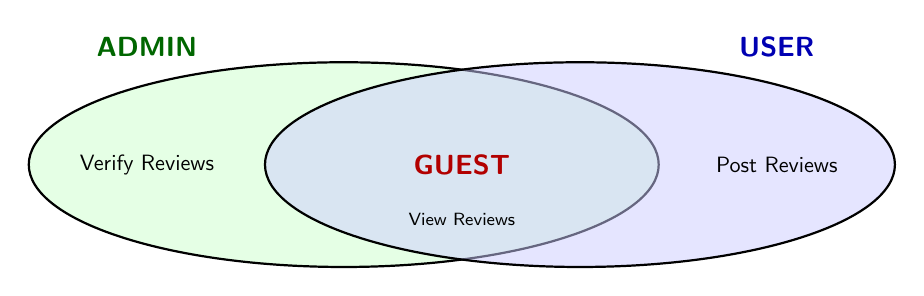
\begin{tikzpicture}[thick, font=\sffamily]
		
		% 1. ADMIN Ellipse (Left - Green)
		\draw[fill=green!20, fill opacity=0.5] (0,0) ellipse (4cm and 1.3cm);
		\node[text=green!40!black] at (-2.5, 1.5) {\textbf{ADMIN}};
		
		% 2. USER Ellipse (Right - Blue)
		\draw[fill=blue!20, fill opacity=0.5] (3,0) ellipse (4cm and 1.3cm);
		\node[text=blue!70!black] at (5.5, 1.5) {\textbf{USER}};
		
		% 3. GUEST Label (Placed in the intersection)
		% The intersection center is roughly at (1.5, 0)
		\node[text=red!70!black] at (1.5, 0) {\textbf{GUEST}};
		
		% --- Example Permissions ---
		\node[scale=0.8] at (-2.5, 0) {Verify Reviews}; % Admin Only side
		\node[scale=0.8] at (5.5, 0) {Post Reviews};   % User Only side
		\node[scale=0.8] at (1.5, -0.7) {\footnotesize View Reviews}; % Guest (Intersection)
		
	\end{tikzpicture}
	\caption{Permission Overlap}
	
\end{figure}

To ensure consistency and data integrity, each review follows a standardized structure. Students must complete the following numerical and string fields to submit their feedback:

\begin{itemize}
	\item \textbf{Degree Program}: specific degree course the student is currently enrolled in.
	\item \textbf{Reviewed Course}: name of the subject being evaluated.
	\item \textbf{Instructor}: name of the teacher who held the course.
	\item \textbf{Year of Completion}: academic year in which the course was finished.
	\item \textbf{Rating}: numerical value representing the student's assessment.
	\item \textbf{Comment}: text field for providing detailed qualitative feedback.
\end{itemize}

\subsection{System architecture and tools}


